\documentclass{article}
\usepackage{graphicx}
\usepackage[spanish]{babel}
\usepackage[utf8]{inputenc}
\usepackage{float}
\usepackage{amsmath}

\title{Procesos reversibles, entropía y probabilidad}
\author{}
\date{}

\begin{document}
\maketitle

\section{Reversibilidad de procesos termodinámicos}
Cuando un proceso termodinámico evoluciona de un estado de equilibrio inicial a
otro final, \textbf{pasando a través de infinitos estados de equilibrio}, se
dice que el proceso es reversible.

Ahora, consta definir qué es un estado de equilibrio; para ejemplificar:
digamos que tenemos un émbolo y aplicamos presión a temperatura constante, de
forma que modificamos su volumen. Este proceso pasa por infinitos estados de
equilibrio, ya que las variables termodinámicas se equilibran en cualquier
punto en que nosotros dejemos de aplicar presión.

Un sistema se encuentra en equilibrio termodinámico si, sometido a
determinadas condiciones de contorno (impuestas desde el medio) \textbf{el
    sistema no experimenta ningún cambio espontáneo de estado}.

En el ejemplo anterior, al aplicar presión al émbolo se reduce el volumen del
gas, pero una vez detenida la acción externa, el sistema permanece en reposo:
no ocurre ninguna transformación espontánea. Las variables se ajustan de
acuerdo con las relaciones termodinámicas del sistema (por ejemplo, un aumento
de presión conlleva una disminución de volumen).

Para hablar de reversibilidad, es necesario que el sistema pase por infinitos
estados de equilibrio, de esa manera podemos recorrer un ciclo cerrado.
Recorrer un ciclo cerrado implica que, dado un estado inicial $A$ y otro $B$,
podemos pasar de el estado $A$ al $B$ y luego volver al estado $A$; el camino
que sigamos para lograr esto es indiferente.

\begin{figure}[H]
    \centering
    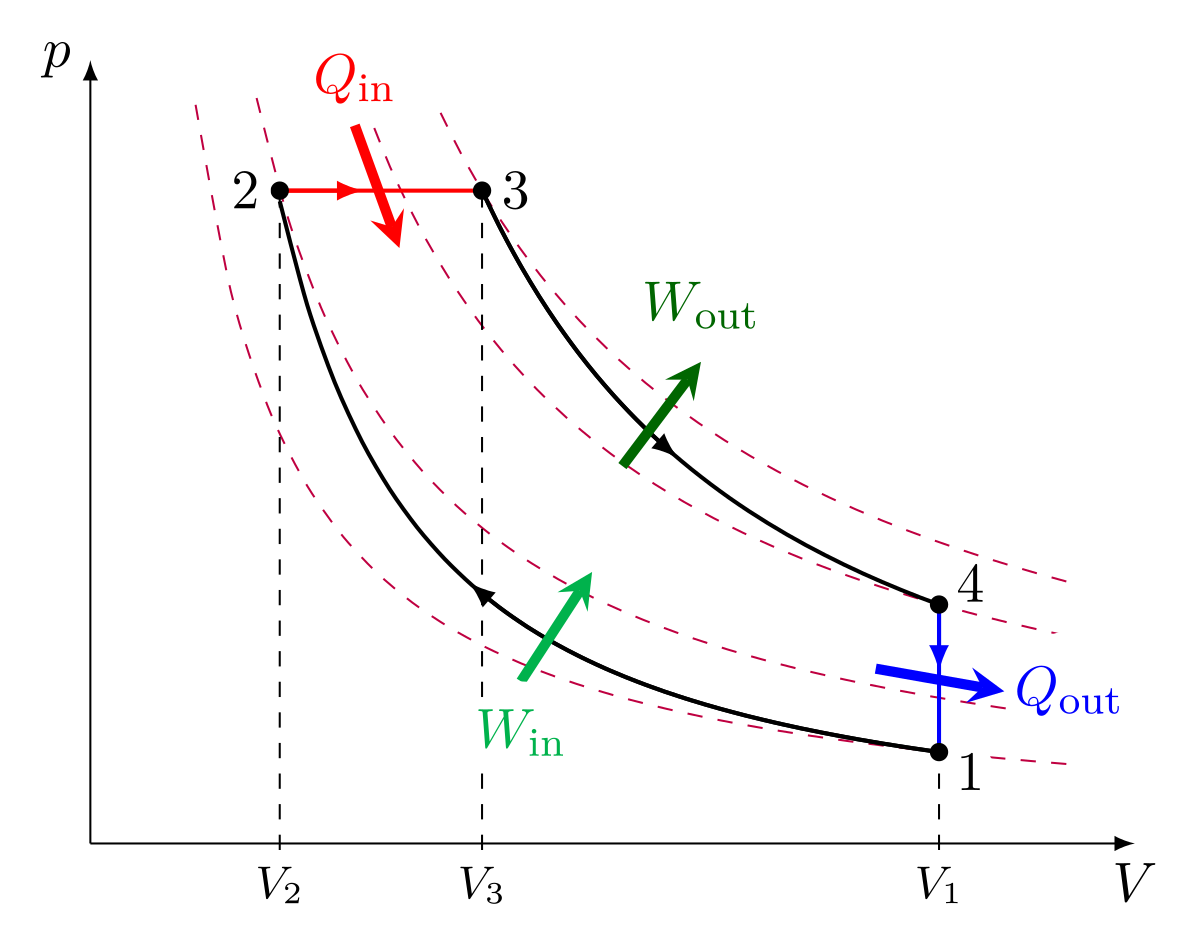
\includegraphics[width=300px]{Diagrama_PV_del_Ciclo_de_Diesel.svg.png}
    \caption{Diagrama P-V de un ciclo térmico (ej. ciclo Diesel)}
\end{figure}

En el diagrama de la Figura 1 se muestra un ciclo termodinámico donde el gas
atraviesa diversas transformaciones:
\begin{enumerate}
    \item De 1 a 2: compresión adiabática (se realiza trabajo sobre el gas).
    \item De 2 a 3: expansión a presión constante (recepción de calor).
    \item De 3 a 4: expansión adiabática (el gas realiza trabajo).
    \item De 4 a 1: enfriamiento a volumen constante (isocórico).
\end{enumerate}

Este ciclo lo puede recorrer de forma indeterminada ya que todas las
transformaciones son reversibles. Podemos ver entonces que el gas experimenta
una compresión, aumento de calor, ejerce un trabajo y se enfría. Este es el
principio de funcionamiento de un motor diesel; estamos comprimiendo el gas
para hacer que explote y entregue trabajo.

\subsection{Reversibilidad}
Como ya vimos, la reversibilidad implica que el sistema pase por infinitos
estados de equilibrio. De esta manera, un sistema reversible puede cambiar a un
estado y volver a su estado original sin sufrir cambios. Podemos ver entonces
que el cambio de la energía interna de un sistema que recorre un ciclo $A\to B
    \to A$ es nulo
\begin{equation}
    \Delta U_{ABA} = 0
\end{equation}

\begin{figure}[H]
    \centering
    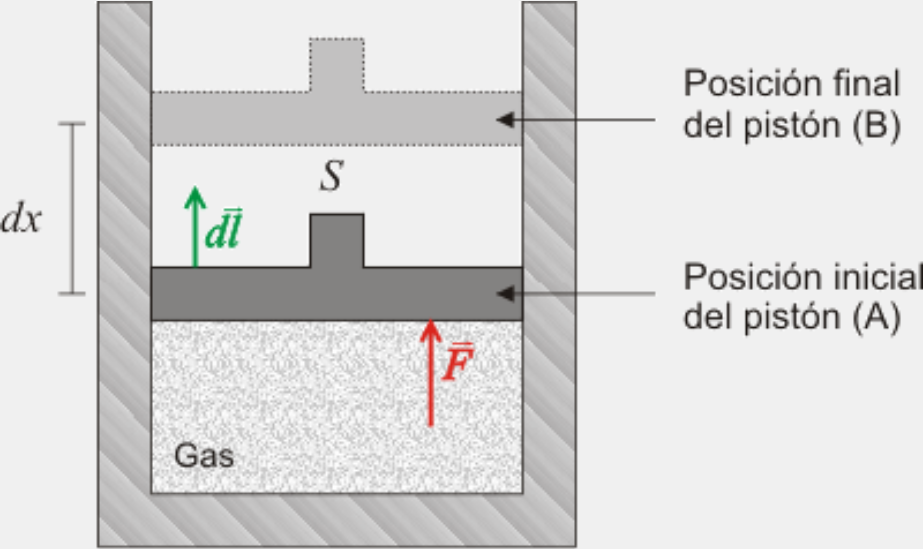
\includegraphics[width=300px]{embolo-gas.png}
    \caption{Émbolo con un gas que realiza trabajo sobre el medio}
\end{figure}

La figura 2
muestra un émbolo con un gas que realiza un trabajo sobre el medio, una fuerza
$\vec{F}$ que puede ser expresada por su módulo y un vector unitario $\vec{u}$,
así $\vec{F}=F\vec{u}$, y un cambio en la posición del pistón $\vec{dl} =
    \vec{u}dx$. La definición de trabajo está dada por
\begin{equation}
    W_{AB} = \int_{A}^{B}{\vec{F}\vec{dl}} = \int_{A}^{B}{F(\vec{u}
    \cdot\vec{u})dx} = \int_{A}^{B}{Fdx}
\end{equation}
Ahora, la definición de presión
\begin{equation}
    p=\frac{F}{S}
\end{equation}
nos sirve para expresar el trabajo como
\begin{equation}
    W_{AB} = \int_{A}^{B}{pS\,dx} = \int_{V_A}^{V_B}{p dV}
\end{equation}
Ya que $Sdx$ es un cambio infinitesimal del volumen, o sea, $dV$.

Ahora un trabajo realizado en un ciclo
\begin{equation}
    \begin{split}
        W_{ABA} &= \int_{V_A}^{V_B}{p_1(V) dV} + \int_{V_B}^{V_A}{p_2(V) dV}
        \\[1em]
        &= \int_{V_A}^{V_B}{p_1(V) dV} - \int_{V_A}^{V_B}{p_2(V) dV}
    \end{split}
\end{equation}
Nótese que las presiones son distintas, sino el trabajo neto sería cero. Ahora,
depende de como recorremos el camino, el trabajo será negativo o positivo si
asumimos que $p_1(V) > p_2(V)$ para todo valor de $V$. Para ser más específicos
con la notación, el trabajo es una integral de línea cerrada
\begin{equation}
    W = \oint p\, dV
\end{equation}
donde integramos en una forma diferencial (1-forma) en un plano dado por
$(V,p)$, no en un campo vectorial.

\subsection{Funciones de estado}
Tanto el trabajo como el calor en un sistema dependen de la transformación que
sufre el mismo. Se define a una función de estado como una propiedad de un
sistema termodinámico que depende sólo del estado del sistema, y no de la
\textbf{forma} en que el sistema llegó a dicho estado.

Así, el calor y la temperatura \textbf{no son funciones de estado}. En cambio,
la \textbf{entropía} y la energía interna son funciones de estado.
No dependen del tipo de transformación que sufre el sistema. Son propiedades
intrínsecas del sistema.

Las funciones que no son de estado pueden verse como procesos en los cuales las
funciones de estado cambian. Por ejemplo al aumentar el calor, la entropía
aumenta.

\section{Segundo principio}
El primer enunciado del segundo principio nos habla de que no todo el calor
puede ser transformado en trabajo de forma íntegra:
``No es posible ninguna transformación cíclica que transforme íntegramente el
calor absorbido en trabajo'' (Enunciado de Kelvin-Planck).

Así obtenemos que $\Delta U = 0$ y, por lo tanto $Q = W$. Si tenemos en cuenta
que una máquina térmica utiliza un calor $Q_1$ para realizar un trabajo $W$ y
cede un calor $Q_2$, entonces
\begin{equation}
    Q_1 + Q_2 = W \Rightarrow W = Q_1 - |Q_2|
\end{equation}
Colocamos el valor absoluto ya que $Q_2$ siempre será negativo al ser el calor
de salida.

\subsection{Rendimiento ($\eta$)}
El rendimiento es la relación entre trabajo producido y el calor entregado.
Teniendo en cuenta el enunciado de Kelvin-Planck sabemos que éste rendimiento
siempre será menor que 1.
\begin{equation}
    \eta = \frac{W}{Q_1} \qquad W < Q_1 \implies \eta < 1
\end{equation}
Usando la expresión de trabajo anterior obtenemos
\begin{equation}
    \eta = \frac{Q_1 + Q_2}{Q_1} = 1 + \frac{Q_2}{Q_1} = 1 - \frac{|Q_2|}{Q_1}
\end{equation}

\subsection{Refrigerador}
El enunciado de Clausius del segundo principio de la termodinámica, nos dice
que ``No es posible el paso de calor de un cuerpo frío a uno caliente sin el
consumo de trabajo''. Para ello, si necesitaramos enfríar un cuerpo, es decir,
transferir calor de un cuerpo frío a uno caliente (por ejemplo, tu heladera
puede estar a unos 6 grados centígrados, mientras que el medio a unos 30 grados
centígrados), necesitaremos ejercer un trabajo. Como un refrigerador trabaja en
ciclos, tenemos que la energía interna es nula, por lo que de nuevo
\begin{equation}
    W = Q_1 + Q_2 \implies |Q_1| - |W| = Q_2
\end{equation}
Ya que $W < 0$ y $Q_1 < 0$ son trabajo entregado al refrigerador y calor cedido
al medio.

\subsection{Eficiencia ($\epsilon$)}
Un refrigerador optimizará reduciendo el trabajo condumido para la misma
cantidad de calor extraída.
\begin{equation}
    \eta = \frac{Q_2}{|W|}
\end{equation}
Donde $W\ne 0$, así $\eta < \infty$.


\end{document}